
%%%%%%%%%%%%%%%%%%%%%%%%%%%%%%%%%%%%%%%%%%%%%%%%%%%%%%%%
% LaTex Template for proposals within the              %
% DFG Research Unit Program                            %         
%Planet Formation Witnesses and Probes: Transition Discs
% August 2016                                            %                           
%                                                      %
%%%%%%%%%%%%%%%%%%%%%%%%%%%%%%%%%%%%%%%%%%%%%%%%%%%%%%%%
%
% 
%
% This template may be used to prepare proposals in latex.
%
%
% The project description, including publication list, should be no more than 20 pages
% in length. It should be self-explanatory and not require reviewers to read the 
% literature that is quoted or enclosed.

\documentclass[10pt,fleqn,twoside]{article}

%%%%%%%%%%%%%%%%% GET THE STYLE STUFF %%%%%%%%%%%%%%%%%%%

%%%% USE ARIAL FONT %%%%%%%%%%%%%%%%%%%%%%%%%%%%%%%%%%%%%%%%%%%%%%%%%%%%%%
\usepackage{helvet}
\renewcommand\familydefault{phv}

%%%% INCLUDE NECESSARY PACKAGES %%%%%%%%%%%%%%%%%%%%%%%%%%%%%%%%%%%%%%%%%%
%\usepackage{babel}
\usepackage[UKenglish]{babel}
\usepackage{amsmath}
\usepackage{amssymb}
\usepackage{fancyhdr}
\usepackage{natbib}
\usepackage{ae,aecompl}
\usepackage{graphicx}
\usepackage{palatino}
\usepackage[T1]{fontenc}
\usepackage[right]{eurosym}
\usepackage{rotating}
\usepackage{epsf}
\usepackage{setspace}
\usepackage{xspace}
\usepackage{multicol}
\usepackage{siunitx}
%\usepackage{caption}

\usepackage{sfmath}

\usepackage[utf8]{inputenc}

% ========= hyperref & Colors & Links ===========
\usepackage[usenames,dvipsnames]{xcolor}
%\usepackage[breaklinks]{hyperref}
\usepackage{hyperref}
\addto\extrasUKenglish{%
\def\sectionautorefname{Section}%
\def\subsectionautorefname{Section}%
\def\subsubsectionautorefname{Section}%
\def\paragraphautorefname{Section}%
}
\usepackage[all]{hypcap} % fixes links to floats
\usepackage{aas_macros}  %
\setlength{\bibsep}{-0.5pt}

% ========= highlighting important parts of the proposal ===========
\definecolor{HighLight}{rgb}{0.9,0.3,0.0}
%\newenvironment{highlight}{\color{blue}\itshape}{\ignorespacesafterend}
%\newenvironment{highlight}{\color{RedOrange}\itshape}{\ignorespacesafterend}
%\newenvironment{highlight}{\color{RedOrange}\bfseries}{\ignorespacesafterend}
%\newenvironment{highlight}{\color{BrickRed}\bfseries\itshape}{\ignorespacesafterend}
%\newenvironment{highlight}{\color{BrickRed}\bfseries}{\ignorespacesafterend}
%\newenvironment{highlight}{\color{HighLight}\bfseries}{\ignorespacesafterend}
\newenvironment{highlight}{\color{HighLight}}{\ignorespacesafterend}
\newenvironment{missingenv}{\color{red}}{\ignorespacesafterend}

\definecolor{Emphasize}{rgb}{0.0,0.5,0.0}
\newenvironment{Emphasize}{\color{Emphasize}\itshape}{\ignorespacesafterend}


% strike through comments: to turn them off, uncomment the renewcommands below
\usepackage{soul}
\setstcolor{red}

% ========= Commands specially for the forschergruppe =========

\newcommand{\todo}[1]{\textcolor{red}{\bf #1}}
\newcommand\connect[1]{{\color{OliveGreen} #1}}

%%%% CAPTION LAYOUT %%%%%%%%%%%%%%%%%%%%%%%%%%%%%%%%%%%%%%%%%%%%%%%%%%%%%

\usepackage[font={small}]{caption}

%%%% PAGE LAYOUT %%%%%%%%%%%%%%%%%%%%%%%%%%%%%%%%%%%%%%%%%%%%%%%%%%%%%%%%%
\setlength{\textheight}{22cm}
\setlength{\topmargin}{-1.2cm}
\setlength{\textwidth}{15.6cm}
\setlength{\oddsidemargin}{0.0cm}
\setlength{\evensidemargin}{0.0cm}
\setlength{\mathindent}{1.5cm}
\setlength{\parindent}{0.0cm}
\setlength{\parskip}{0.08cm}

%%%% PAGE HEADER %%%%%%%%%%%%%%%%%%%%%%%%%%%%%%%%%%%%%%%%%%%%%%%%%%%%%%%%%%
\pagestyle{fancy}
\fancyhead[RE,RO]{}
\fancyfoot[RO]{\thepage}
\fancyfoot[LE]{\thepage}
\fancyfoot[CE,CO]{}

%%% FONTS FOR THE TITLE PAGE %%%%%%%%%%%%%%%%%%%%%%%%%%%%%%%%%%%%%%%%%%%%%%
\newfont{\tpfonta}{cmssbx10 scaled 1600}
\newfont{\tpfontb}{cmssbx10 scaled 3200}

%%%% COLOR DEFINITIONS %%%%%%%%%%%%%%%%%%%%%%%%%%%%%%%%%%%%
\definecolor{blue} {rgb} {0.25,0.25,0.75}

%%%% ADDITONAL EMPHASIS %%%%%%%%%%%%%%%%%%%%%%%%%%%%%%%%%%%
\newcommand{\cem}{\color{blue}}
\newcommand{\eem}{\sl\color{blue}}

%%%% BIBTEX PUNCTUATION %%%%%%%%%%%%%%%%%%%
\bibpunct{(}{)}{;}{a}{}{,} % to follow the A&A style

%%%% SET THE COLOR OF THE (SUB-) SECTION TITLES %%%%%%%%%%% 
\newcommand{\Tcol}{\color{blue}}

%%%% SET THE COLOR OF THE TITLE BOX BACKGROUND %%%%%%%%%%%%
\definecolor{Background}{rgb} {0.62,0.75,0.5}

%%%%%%%%%%%%%% REFERENCE SECTION NAME %%%%%%%%%%%%%%%%%%%%
\renewcommand\refname{\Tcol 9. Bibliography}

%%%%%%%%%%%%%% NICER PROJECT REFERENCES %%%%%%%%%%%%%%%%%%%

\newenvironment{literature}%
 {\begin{multicols}{2}\begin{scriptsize}\begin{list}{}{%
   \setlength{\topsep}{0em}%
   \setlength{\parskip}{0em}%
   \setlength{\parsep}{0em}%
   \setlength{\itemsep}{0em}%
   \setlength{\rightmargin}{0em}%
   \setlength{\leftmargin}{2em}%
   \setlength{\itemindent}{-2em}}}%
 {\end{list}\end{scriptsize}\end{multicols}}

%
% ...A compact itemize environment
%
\newenvironment{compactitemize}%
 {\begin{list}{$\bullet$}{%
   \setlength{\topsep}{0em}%
   \setlength{\parskip}{0em}%
   \setlength{\parsep}{0em}%
   \setlength{\itemsep}{0.0\baselineskip}%
   \setlength{\rightmargin}{0em}%
   \setlength{\leftmargin}{2.0em}%
   \setlength{\labelsep}{0.5em}%
   \setlength{\labelwidth}{1em}%
}}
 {\end{list}}

\newcounter{qcounter}
\newenvironment{compactenumerate}%
 {\begin{list}{\arabic{qcounter})~}{\usecounter{qcounter}%
   \setlength{\topsep}{0em}%
   \setlength{\parskip}{0em}%
   \setlength{\parsep}{0em}%
   \setlength{\itemsep}{0.0\baselineskip}%
   \setlength{\rightmargin}{0em}%
   \setlength{\leftmargin}{2.0em}%
   \setlength{\labelsep}{0.5em}%
   \setlength{\labelwidth}{1em}%
}}
 {\end{list}}

%%%% EXPLANATION FOR THE CONNECT COLOR %%%%%%%%%%% 
\newcommand{\footexplainconnect}{\footnote{The text highlighted in \connect{green} refers to the connection of this project to other projects of this Research Unit.}}
 
%%%%%%%%%%%%%%%%%% NICER REFERENCES %%%%%%%%%%%%%%%%%%%

%\usepackage[capitalise,nameinlink]{cleveref}
\newcommand{\cref}[1]{\autoref{#1}}

%%%%%%%%%%%%%%%%%% COLOR THE SECTION NUMBERS %%%%%%%%%%%%%%%%%

\makeatletter
\renewcommand\@seccntformat[1]{\color{blue} {\csname the#1\endcsname}\hspace{0.5em}}
\makeatother
\renewcommand\thesection{\arabic{section}.}
\renewcommand\thesubsection{\arabic{section}.\arabic{subsection}}

%%%%% color sections
\usepackage{sectsty}
\allsectionsfont{\color{blue}}


%%%% CHANGE THE APPEARANCE OF THE \PARAGRAPH COMMAND  %%%%%%%%%%%%%%%%%%%%%%%%%%%%%%%
\makeatletter
\renewcommand\paragraph{\@startsection{paragraph}{4}{\z@}%
            {-2.5ex\@plus -1ex \@minus -.25ex}%
            {1.25ex \@plus .25ex}%
            {\normalfont\normalsize\bfseries\Tcol}}
\makeatother
\setcounter{secnumdepth}{4}     % how many sectioning levels to assign numbers to
\setcounter{tocdepth}{4}        % how many sectioning levels to show in ToC

%%%%% set header

\renewcommand{\sectionmark}[1]{\markright{\color{black}#1}}

\newcommand{\caphighlight}[1]{{\bf #1}}



%%%%%%%%%%%%%%%%% DEFINE THE HEADER TEXT %%%%%%%%%%%%%%%%

\fancyhead[LE,LO]{\slshape
%%%%  Please edit
%
Cornelis Dullemond and Wilhelm Kley: RU Transition Discs Project Description}
%
%
%%%%%

\begin{document}


\newpage

%%%% PROJECT DESCRIPTION STARTS HERE %%%%%%%%%%%%%%%%%%%%%%%%%%%%%%%%%%%

\setcounter{page}{1}

\centerline{\huge\bf\Tcol
%
%
%
%
%%%%  Please edit
%
 Project D2:}
\vspace{1em}

\centerline{\LARGE\bf\Tcol Origin of complex non-axisymmetric structures}\vspace{0.3em}
\centerline{\LARGE\bf\Tcol in type 2 transition disks}

%
%%%%
%
%
%
%
\vskip1.0cm

%%%%  Please edit

\noindent{\bf Authors:}\\
\begin{tabular}{ll}
{\textsf{PI:}}                 & C.P.~Dullemond (Heidelberg)\\
{\textsf{Co-I:}}               & W.~Kley (T\"ubingen)\\
{\textsf{Collaborations:}}     & L.~Testi (ESO), B.~Ercolano (USM), E.~van Dishoeck (MPE), T.~Henning (MPIA)\\
\end{tabular}

\todo{Check if all are part of the proposal.}
\todo{Links to other projects.}

%%%%  Please edit

\vspace{1em}
\noindent{\bf Requested positions: 1 Postdoc} \\

\vspace{1em}
\noindent{\bf Abstract:}\\
Transition disks have recently been shown to display spectacular structures
such as large scale spirals, blobs, tilts etc. These features indicate that
highly dynamic processes are going on in these disks, allowing us to test
our understanding of the physics of protoplanetary disks. This project aims
to understand these structures in terms of dynamic models of disks.


\section{State of the art and preliminary work}
\renewcommand{\leftmark}{\sc State of the Art and preliminary work}
With the spectacular new capabilities of observatories in the millimeter
wavelength range (ALMA) and at optical wavelengths (Subaru and VLT
coronographic imagers, most recently: VLT-SPHERE), protoplanetary disks are
found to be much more complex than previously thought. Until only a few
years ago observations of protoplanetary disks were consistent with the idea
of them being mostly axi-symmetric rotating structures around young stars.  

Recent observations have now shown this picture to be false, in particular
for transition disks. Many such disks, while remarkable in their own right
due to their large inner holes (see project {\bf D1}), are even more
remarkable due to their often-present strong deviations from axisymmetry. At
millimeter wavelengths, spatially resolved with ALMA, all transition disks
show a strong dust emission ring just beyond the inner hole. Several of
them, in particular the sources HD 142527 and Oph IRS 48, show this ring to
be strongly lopsided: one side being clearly much brighter than the other
side \citep{2013Natur.493..191C,2013Sci...340.1199V}. These appear to be
vortices created by the Rossby wave instability \citep{2012MNRAS.419.1701R}.
This raises the exciting possibility that these are {\em dust-trapping
  vortices}, predicted to play an important role in planet formation
\citep{1995A&A...295L...1B,1997Icar..128..213K}.

At optical and near infrared wavelengths many of these sources show another
remarkable and unexpected feature: grand design spiral waves (e.g.~the
sources HD 135344b, MWC 758, HD 100453). While $m=1$ spiral waves were
expected as a result of newborn planets embedded in these disks, the spirals
observed in many Type 2 transition disks are symmetric $m=2$ modes, making
them look like the galaxy M51. The origin of these spirals is still hotly
debated and planetary/stellar companions \citep{2016ApJ...816L..12D} and
gravitational instabilities \citep{2016arXiv161109361T} are often suggested
to be at their origin, as is residual infall into the disk
\citep{2015A&A...582L...9L}. Recently an even more unorthodox and intriguing
scenario was proposed: The bright ring of scattered light (the illuminated
inner rim of the outer disk as seen with the Subaru and VLT telescopes) of
HD 142527 has two conspicuous dark spots on almost opposite
sides. \citet{2015ApJ...798L..44M} were able to show with 3-D radiative
transfer modeling that these dark spots are most likely the shadows cast by
an inclined small inner disk. If this scenario is confirmed, HD 142527 (and
possibly HD 100453 and other transition disks) is an "inclined disk inside a
disk" (a warped disk). According to \citet{2016ApJ...823L...8M} these two
shadows on opposite sides of the bright rim may even be the origin of the
$m=2$ spiral waves, caused by the brief loss of pressure in these shadows.
This is an intriguing possibility, as it would indicate that Type 2
transition disks may be related to warped disks, and perhaps be the origin
of the misalignment effects seen in many exoplanetary systems with the
Rossiter-Mclaughlin effect.

But how can the inner disk have a different rotation axis as the outer one?
Is this a result of an inclined planet or brown dwarf orbiting inside the
gap? For HD142527 a companion star is known to exist, but it is at the
current epoch still rather close to the main star compared to the size of
the cavity, so it is not directly clear that this companion is responsible
for the large cavity. Or is this due to late accretion of different angular
momentum molecular cloud material? \citet{2011MNRAS.417.1817T} suggest this
scenario to explain misaligned exoplanetary systems. It might also explain
misaligned outer disks. Or could the Kozai-mechanism caused by a companion
at large radii cause this?

These enigmatic non-axisymmetries in Type 2 TDs offer a unique opportunity
to test our understanding of the physical processes occurring in these
disks. The features appear to be highly organized, not random. This suggests
that a strong and well-defined physical mechanism is at work. If we identify
this mechanism (or these mechanisms), we do not only solve the mystery of
these non-axisymmetric features, but also get a better understanding of the
dominant physical processes at work in these disks. It is hoped that this
may allow us to get a better understanding of the process of planet
formation.  For instance, several attempts have been made to explain the
spiral structures by embedded planets \citep{2012ApJ...748L..22M,
  2015A&A...578L...6B, 2015MNRAS.453.1768P}, though it turns out that
planetary spiral features are usually single-armed ($m=1$) instead of the
double-armed ($m=2$) spirals often seen. Also the giant central cavity of
Type 2 TDs were investigated in the context of gap-opening planets, though
it turns out that this is not easy and requires at least multiple planets to
work \citep{2011ApJ...729...47Z}. The bright dust rings with often lopsided
geometry seen in Type 2 TDs strongly suggest dust trapping at work. These
rings are consistent with the radial dust trapping suggested by
\citet{1972fpp..conf..211W}, and the lopsidedness appears to be a result of
dust trapping in a huge vortex \citep{1995A&A...295L...1B,
  1997Icar..128..213K, 2013A&A...550L...8B, 2013A&A...553L...3A,
  2014ApJ...795...53Z, 2016MNRAS.458.3927B}. What is the origin of these
dust traps remains unsolved. \citet{2012MNRAS.419.1701R} suggest that this
is a result of a change in viscosity in the disk at the outer edge of the
``dead zone''.  They find not only a strong ring-shaped pressure bump
forming (which can trap dust), but they see this ring also periodically
becoming lopsided by forming a giant anti-cyclonic vortex. The formation of
such vortices was first reported by \citet{1999ApJ...513..805L}, and it
seems that with Type 2 TDs we now see evidence for their existence. Given
that dust tends to get trapped in these vortices, an exciting question is
whether these vortices are the birthplaces of new planets.

The goal of this proposal is to attemp to understand the non-axisymmetric
features in Type 2 TDs from the perspective of gas dynamics. Particular
emphasis will be put on ``non-standard'' dynamics such as out-of-plane
companions, secondary infall and shadow-driven dynamics. Ultimately we wish
to find out if Type 2 TDs are oddballs or not, and if they teach us
something about the formation of planets or are too exotic to do so.


\subsection{Preliminary work}
As a preparation for this project we have conducted several small
preliminary investigations in the context of Bachelor projects. We are also
involved in several collaborations involving VLT-SPHERE scattered light
images of Type 2 TDs as well as ALMA observations.

\subsubsection{VLT-SPHERE observations of Type 2 TDs}
Th.~Henning, one of the collaborators on this project, is involved in
VLT-SPHERE scattered light image observations of Type 2 TDs. A particularly
spectacular example, where the PI was also involved in, is the very recent
image of the Type 2 TD HD 100453 \citep{2016arXiv161010089B}. This is a
Transition Disk with an inner disk spanning out to 1 AU, and an outer disk
spanning between 20 AU and 45 AU. It features a prominent $m=2$ spiral
pattern originating from a bright ring that features two bright arcs
(presumably due to the scattering phase function) and two dark spots
(presumably due to the shadowing caused by an inclined inner disk, as in HD
142527 \citep{2015ApJ...798L..44M}). The observed polarized intensity
and the synthetic model image are shown in Fig.~\ref{fig-benisty}. The
synthetic image was made with the MCMax radiative transfer code, and
the setup involved in tilted inner disk that produced the shadow features
on the ring, and parameterized spiral features.

\begin{figure}
\centerline{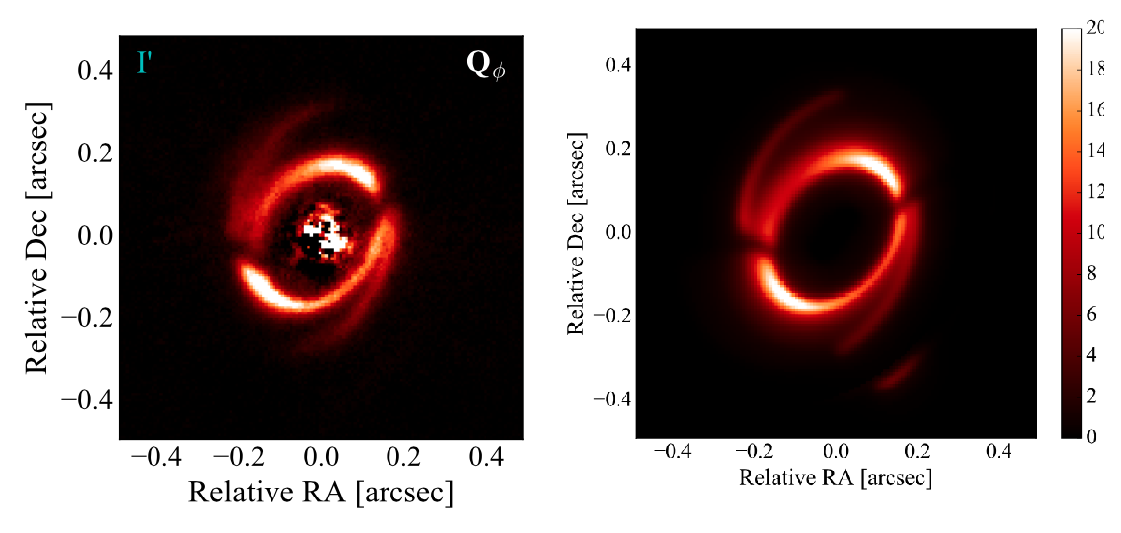
\includegraphics[width=0.95\textwidth]{D2Fig/Benisty.eps}}
\caption{\label{fig-benisty} Polarized scattered light observations of the
  Type 2 TD HD100453. \caphighlight{Left:} Actual observations with
  VLT-SPHERE in the I' band. \caphighlight{Right:} Synthetic model image
  made with the MCMax Monte Carlo code. From: \citet{2016arXiv161010089B}.}
\end{figure}

\subsubsection{ALMA observations of Type 2 TDs}
Dr.~Akimasa Kataoka has been a postdoc at the ITA since April 2015 on his
own JSPS-Fellowship grant. During this period he successfully applied for
substantial ALMA time to observe the Type 2 TD source HD 142527 using the
newly available polarization mode. The observations we obtained have turned
out to be quite spectacular (Fig.~\ref{fig-kataoka}). The strongly lopsided
arc-shaped dust emission was already well known since
\citep{2013Natur.493..191C}. But the shape of the polarized light image
contains a huge amount of additional information. Please note that it is not
the purpose of this project to investigate how to use this new technique of
polarized thermal emission at millimeter wavelengths. This is the topic of
another -- completely separate -- DFG proposal that was submitted in the
summer of 2016 (DFG DU 414/17-1). Here we merely show the kind of objects we
study and the type of observations we are involved in, which will (in
addition to published data from other groups) serve as observational
evidence for the complex disk geometries seen in Type 2 TDs.

\begin{figure}
\centerline{\includegraphics[width=0.95\textwidth]{D2Fig/Kataoka.eps}}
\caption{\label{fig-kataoka} ALMA Observations of the Type 2 TD HD 142527.
  \caphighlight{Left:} The continuum (Stokes I component) at 850 $\mu$m
  showing the well known arc-shaped structure believed to be dust trapped in
  a Rossby-vortex.  \caphighlight{Right:} The polarized intensity with the
  polarized direction overlayed.  From: \citet{2016ApJ...831L..12K}.}
\end{figure}

The PI has also been involved in an ALMA observational study of the source
IRS 48 from the team of Ewine van Dishoeck, where an even stronger lopsided
dust emission was found \citep{2013Sci...340.1199V}. 

The PI and collaborators on this project are continuing involvement (and
leading) of such observational campaigns.


\subsubsection{Preliminary models of out-of-plane companion-disk interaction}
Out-of-plane planet disk interaction models have been made by
\citet{2011A&A...530A..41B} and \citet{2013A&A...555A.124B} using a fully
3-D radiation hydrodynamics grid-based code. 
The focus here was on intermediate mass planets inducing moderate
disk warps, and the aim was to understand inclination damping and
migration. Other work include \citet{2013MNRAS.431.1320X} who employ
a Smooth Particle Hydrodynamics code to study the effect of such an
inclined companion on the disk structure, and back on the planet. Also
here the planet mass was intermediate and the induced warps were moderate.
 
For the present purpose we need to go to more extreme cases: higher
inclinations, higher planet masses, and focusing on the change of the
appearance of the disk shape to be able to compare this with observed Type 2
TDs.

As a preliminary test case for such modelling, we performed a set of simple
models using the Smooth Particle Hydrodynamics code Gadget-2. We set up an
initially smooth planar disk, but add a low mass companion on an inclined
circular orbit. The orbit crosses the disk twice each orbital period. The
results of one such model is shown in Fig.~\ref{fig-herbst-6}. As time
passes by, this process opens up a strong gap in the disk. The gravitational
torque of the planet on the inner and outer disk, however, cause both to
precess. The inner disk precesses faster than the outer disk. As a result,
the inner and outer disks become tilted with respect to each other (they are
no longer co-planar). The ``warp'' can be seen in all three panels of
Fig.~\ref{fig-herbst-6}, but the tilt between inner and outer disk is only
seen in the middle panel, which is a snapshot at 50000 years. This model was
initially set up by Dr.~Daniel Harsono and further developed and applied by
Matthew Herbst during his Bachelor thesis project. These results show that
for a brief period the inclined companion can lead to tilted inner/outer
disks, but eventually the outer disk aligns with the plane of the planetary
orbit, and the inner disk disappears by viscous accretion. This viscous
accretion appears to be strongly boosted by excessive numerical viscosity
due to too few SPH particles. This excessive viscous accretion also appears
to be the cause of the very bright outer disk ring. This is presumably not
realistic, so this simulation can merely serve as a proof-of-concept. Much
higher resolution models have to be made, with more careful testing of the
viscosity of the model.

\begin{figure}
\centerline{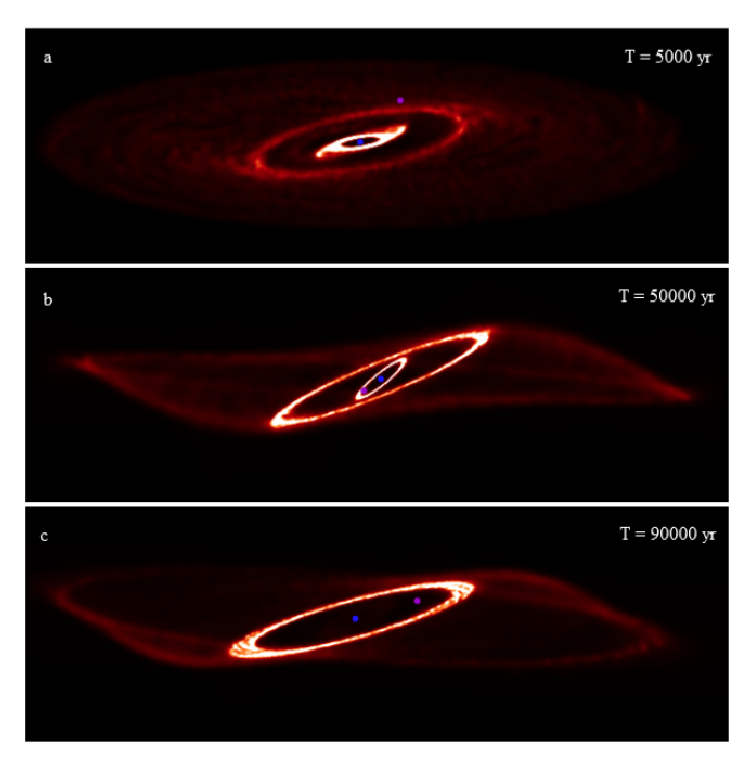
\includegraphics[width=0.8\textwidth]{D2Fig/Herbst_Fig6.eps}}
\caption{\label{fig-herbst-6}Time snapshots of the shape of a circumstellar
  disk disrupted by an inclined planetary companion passing through the disk
  twice each orbit. The star is blue, the planet is purple. The gas SPH
  particles are shown in shades of red (low column density) and yellow (high
  column density). The star has a solar mass. The planet orbital inclination
  is 33 degrees, the semi-major axis 40 AU, the mass 0.01 $M_{\odot}$. The
  disk is initially 200 AU in radius and has a mass of 0.01 $M_{\odot}$. The
  surface density is shown as a projection with respect to a camera. The
  angle of the camera is not the same in each snapshot, but chosen such that
  the warp in the disk is better seen. From: Bachelor Thesis by Matthew
  Herbst, Heidelberg University, 2016.}
\end{figure}



\subsubsection{Preliminary models of secondary disk formation}
As a proof of concept for the secondary accretion of material from a low
mass molecular cloudlet we performed a simple set of grid-based numerical
hydrodynamic models. The model setup is a rectangular grid of 256 $\times$
256 $\times$ 64 cells covering 10 $\times$ 10 $\times$ 2.5 kAU (one kAU =
1000 AU). The initial cloud setup is a simple Gaussian shaped spherical
cloud:
\begin{equation}
\rho({\bf r}) = \rho_0 + (\rho_1-\rho_0)\exp\left(-\frac{|{\bf r}-{\bf r}_{\mathrm{cl}}|^2}{2D^2_{\mathrm{cl}}}\right)
\end{equation}
where $\rho_0$ is the background density, $\rho_1$ is the initial peak
density at the cloud center, ${\bf r}_{\mathrm{cl}}$ is the initial location
of the cloud and $D_{\mathrm{cl}}$ is the cloud initial size. The
temperature is kept constant at all times and locations, such that the sound
speed is 1 $\mathrm{km}/\mathrm{s}$. The gas velocity at all locations in
the grid is initially the same everywhere, but will of course change due to
the gravitational pull of the star and the hydrodynamics of the gas. The
star is kept at a fixed location ${\bf r}_{*}$ at the center of the box, and
the cloud motion has a non-zero impact parameter $b$ with respect to the
star. The gravitational potential of that star was smoothed, but only very
mildly so:
\begin{equation}
  \Phi({\bf r}) = -\frac{GM_{*}}{(|{\bf r}-{\bf r}_{*}|^8+r_{\mathrm{smooth}}^8)^{1/8}}
\end{equation}
The 8th power was chosen to minimize the effect of smoothing on the
solution, essentially limiting the smoothing only to the few cells around
the star. We used a 3-D Riemann-solver hydrodynamics code (developed by the
PI many years ago for the purpose of a lecture on numerical hydrodynamics,
but not public). The main parameters of the model are the size of the cloud
$D_{\mathrm{cl}}$, the initial position of the cloud ${\bf
  r}_{\mathrm{cl}}$, the Mach number of the velocity ${\cal M}$ and the
impact parameter $b$. Using this setup and code, a series of models were
made in the context of the Bachelor thesis of Manuel Kramer during the
summer of 2016. One such model is shown in Fig.~\ref{fig-kramer-4.1}.  This
result shows that such a secondary cloud accretion tends to produce disks
with strong one-armed spiral structure at large scales. Which shape is seen
depends not only on the parameters, but also on the timing of the snapshot.
The geometries can vary a lot. The ones seen in Fig.~\ref{fig-kramer-4.1}
are reminiscent of some geometries seen at large scales around several Type
2 TDs. We also made synthetic scattered light images that can be directly
compared to data. An example is shown in Fig.~\ref{fig-kramer-4.12}. This
image bears resemblance to the arc-shaped envelope around the disk of the
Transition Disk star AB Aurigae as imaged by \citet{1999ApJ...523L.151G}.

\begin{figure}
\centerline{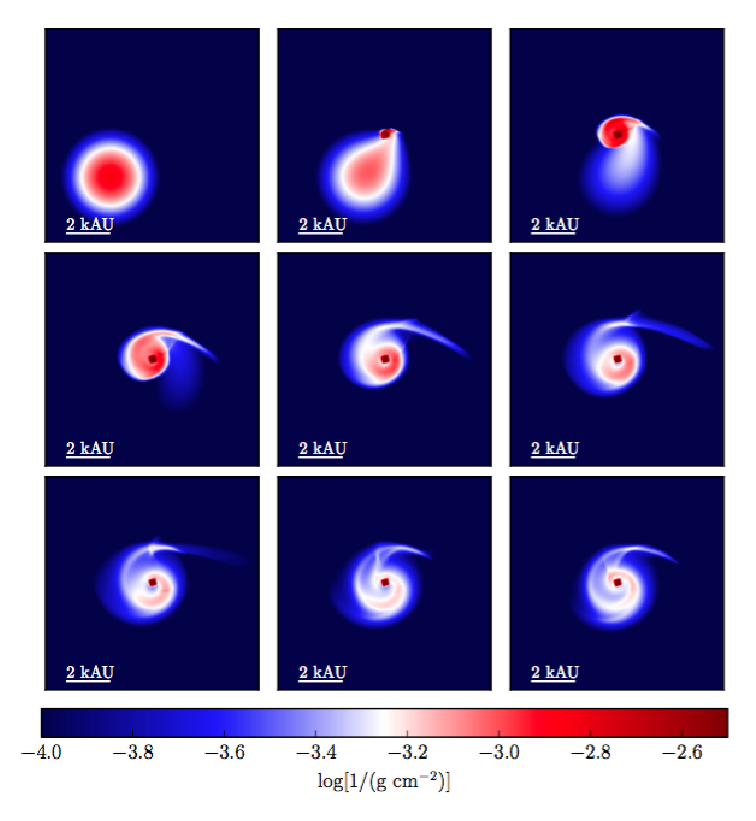
\includegraphics[width=0.9\textwidth]{D2Fig/Kramer_Fig4.1.eps}}
\caption{\label{fig-kramer-4.1}Time sequence of off-center accretion of a
  small low-mass spherical Gaussian molecular cloud by a star. The star is
  at the center, the cloud moves initially from left to right. The star is
  kept fixed, i.e.~the cloud mass is small compared to the star mass. Time
  snapshots (\caphighlight{from left to right, top to bottom}) are with
  $4.8\times 10^3$ years intervals. The color bar is surface density in
  $\mathrm{g}\,\mathrm{cm}^{-2}$. The star mass is 1.4 $M_{\odot}$, the Mach
  number of the cloud velocity with respect to the star. From: Bachelor
  Thesis by Manuel Kramer, Heidelberg University, 2016.}
\end{figure}

\begin{figure}
\centerline{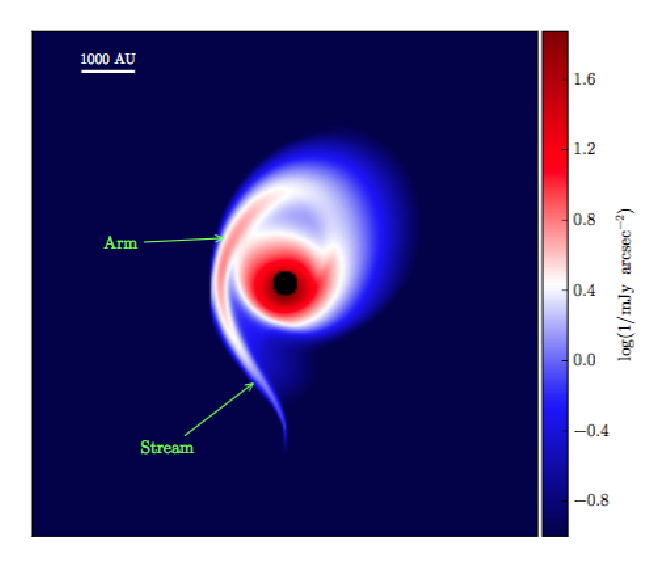
\includegraphics[width=0.5\textwidth]{D2Fig/Kramer_Fig4.12.eps}
\hspace{2em}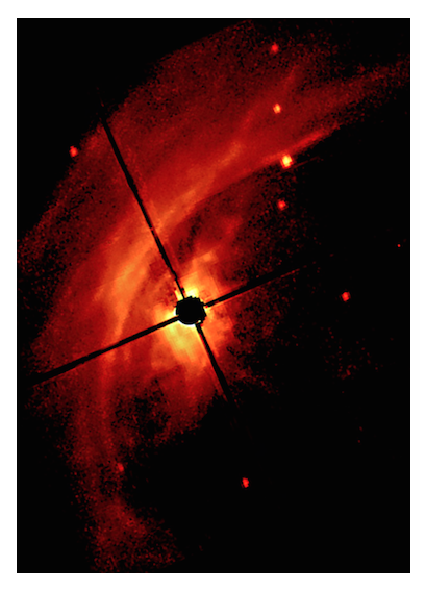
\includegraphics[width=0.3\textwidth]{D2Fig/Kalas.eps}
}
\caption{\label{fig-kramer-4.12}\caphighlight{Left:} Scattered light
  synthetic image computed for a snapshot of the simulations of an
  off-center accretion of a small low-mass spherical Gaussian molecular
  cloud by a star. The color bas unit is mJy/arcsec$^2$. From: Bachelor
  Thesis by Manuel Kramer, Heidelberg University,
  2016. \caphighlight{Right:} Observed scattered light image of the
  arc-shaped envelope around the Type 2 TD star AB Aurigae by P.~Kalas
  \citep{1999ApJ...523L.151G}.}
\end{figure}





\subsection{Project-related publications}

% Please list your own publications related to the proposed project, 
% adhering to the rules of the DFG guidelines 1.91. In brief, please note: 
% - Up to 10 publications
% - The work must be published or accepted.
% - Publications on astro-ph (arXive, SPIRES or articles with a DOI) count as published. 
% - Any work that is only in the status ``accepted'' MUST be attached to the proposal
%    together with the acceptance letter.
% - All publications in this section CAN be attached to the proposal. Please limit these
%    attachments to a minimum and please note that the reviewers may not read the attachments -
%    the proposal has to speak for itself.
% - The number of allowed publications refers to the sum of the publications listed
%    in ``1.1.1 Articles published or officially accepted by publication outlets...'' and 
%    in ``1.1.2 Other publications''. Publications which only exist on public repositories 
%    belong into the category ``Other Publications''.


%\subsubsection{
%Articles published or officially accepted by publication outlets with scientific quality assurance;
%book publications}

\begin{literature}
\item Birnstiel, T., {\bf Dullemond, C.P.} \& Brauer, F., {\em Gas and dust
    evolution in protoplanetary disks}, 2010, A\&A 513, 79. In this paper we
  present the basic code for the evolution of the disk and the dust. The
  disk evolution is followed using the time-dependent viscous disk
  equations, the dust part follows the dust coagulation, fragmentation,
  settling and radial drift of the dust.
% \item S\'andor, Z., Lyra, W., {\bf Dullemond, C.P.}, {\em Formation of Planetary
%     Cores at Type I Migration Traps}, 2011, ApJ, 728, L9. Here we performed
%   detailed N-body calculations of multi-planet systems with migration
%   torques. 
% \item P\'erez, L.M., Carpenter, J.M., Andrews, S.M., Ricci, L., Isella, A.,
%   Linz, H., Sargent, A.I., Wilner, D.J., Henning, T., Deller, A.T.,
%   Chandler, C.J., {\bf Dullemond, C.P.}, Lazio, J., Menten, K.M., Corder, S.A.,
%   Storm, S, Testi, L.  Tazzari, M., Kwon, W., Calvet, N., Greaves, J.S.,
%   Harris, R.J., Mundy, L.G., {\em Spiral density waves in a young
%     protoplanetary disk.}, 2016, Science, 353, 1519. This is the first
%   detection of spiral waves in a protoplanetary disk at millimeter
%   wavelengths.  It shows that these waves are not just surface phenomena,
%   but must be related to actual density waves. 
\item Ataiee, S., {\bf Dullemond, C.P.}, {\bf Kley, W.}, Regaly, Z., \&
  Meheut, H. {\em Planet-vortex interaction: How a vortex can shepherd a
    planetary embryo}, 2014, A\&A, 572, A61. This paper is an example of our
  work on how a planet is interacting with a non-axisymmetric transition
  disk featuring a huge vortex.
\item Ataiee, S., Pinilla, P., Zsom, A., {\bf Dullemond, C.P.}, Dominik, C.,
  \& Ghanbari, J., {\em Asymmetric transition disks: Vorticity or
    eccentricity?}, 2013, A\&A, 553, L3. This paper shows our work on how a
  massive planet can make the disk asymmetric (lopsided) in two independent
  ways: by making the disk eccentric or by creating a vortex. We show how to
  distinguish observationally between these two scenarios. It is an example
  of how we make a link between modeling and observations.
\item M\"uller, T.W.A., \& {\bf Kley, W.}, {\em Modelling accretion in
    transitional disks}, 2013, A\&A, 560, 40.  This paper shows our
  experience with modeling the dynamics of transition disks. In this paper
  the gas flow through the planet-induced gap is studied, which is very
  relevant for the type 2 TDs which usually still have substantial accretion
  onto the star and have inner disks. 
\item D.~Thun, R.~Kuiper, F.~Schmidt, {\bf W.~Kley}, {\em Dynamical friction
    for supersonic motion in a homogeneous gaseous medium}, 2016, A\&A, 589,
  A10. Since we will be dealing with extremely inclined companions
  interacting with the disk in part of this project, the experience gained
  in this paper will be used.
\item Bitsch, B., \& {\bf Kley, W.}, {\em Evolution of inclined planets in
    three-dimensional radiative discs}, 2011, A\&A, 530, 41. This paper
  shows our experience with modeling out-of-plane 3-D planet-disk
  interaction. This paper focused mostly on how the disk damps the
  inclination of the planet, and focused on small inclinations and masses
  lower than about half a Jupiter mass. In this proposal we will shift our
  attention to more extreme cases, as suggested by the large observed disk
  tilts of up to 70 degrees, and focus on how the disk shape is changed as
  a result. 
\item {\bf Kley, W.}, \& Dirksen, G., {\em Disk eccentricity and embedded
    planets}, 2006, A\&A, 447, 369. This was the original paper
  demonstrating how a massive planetary companion can make a disk eccentric.
\item N.~van der Marel, E.F.~van Dishoeck, S.~Bruderer, T.~Birnstiel,
  P.~Pinilla, {\bf C.P.~Dullemond}, T.A.~van Kempen, M.~Schmalzl,
  J.M.~Brown, G.J.~Herczeg, G.S.~Mathews, V.~Geers, {\em A Major Asymmetric
    Dust Trap in a Transition Disk}, 2013, Science, 340, 1199. This was the
  first discovery paper of a dust trapping vortex, and still is the best
  example of such an object so far. The role of the PI was the
  interpretation of the discovered lopsided dust clump as evidence for a
  dust-trapping vortex.
\item M.~Benisty, T.~Stolker, A.~Pohl, J.~de Boer, G.~Lesur, C.~Dominik,
  {\bf C.P.~Dullemond}, M.~Langlois, M.~Min, K.~Wagner, T.~Henning,
  A.~Juh{\'a}sz, P.~Pinilla, S.~Facchini, D.~Apai, R.~van Boekel, A.~Garufi,
  C.~Ginski, F.~M{\'e}nard, C.~Pinte, S.P.~Quanz, A.~Zurlo, A.~Boccaletti,
  M.~Bonnefoy, J-L.~Beuzit, G.~Chauvin, M.~Cudel, S.~Desidera, M.~Feldt,
  C.~Fontanive, R.~Gratton, M.~Kasper, A.M.~Lagrange, H.~LeCoroller,
  D.~Mouillet, D.~Mesa, E.~Sissa, A.~Vigan, J.~Antichi, T.~Buey, T.~Fusco,
  D.~Gisler, M.~Llored, Y.~Magnard, O.~Moeller-Nilsson, J.~Pragt,
  R.~Roelfsema, J-F.~Sauvage, F.~Wildi, {\em Shadows and spirals in the
    protoplanetary disk HD 100453}, 2016, A\&A in press. This is the paper
  presenting the spectacular scattered light image of HD 100453 with the
  ring, the two shadows and the two perfect spirals (the SPHERE image shown
  in Fig.~\ref{fig-benisty}). The PI is closely associated with several
  members of the SPHERE consortium who made this observation, and is
  co-author of this paper having contributed theoretical interpretations.
\item A.~Kataoka, T.~Tsukagoshi, M.~Momose, H.~Nagai, T.~Muto, {\bf
    C.P.~Dullemond}, A.~Pohl, M.~Fukagawa, H.~Shibai, T.~Hanawa,
  K.~Murakawa, {\em Submillimeter Polarization Observation of the
    Protoplanetary Disk around HD 142527}, 2016, ApJ, 831, L12. This paper
  shows the power of ALMA observations of lopsided disks.
\end{literature}

%\subsubsection{Other publications}

%--

% \subsubsection{Patents}
% 
% \paragraph{Pending}
% 
% [Text]
% 
% \paragraph{Issued}
% 
% [Text]

\section{Objectives and work programme}
\renewcommand{\leftmark}{\sc Objectives and work programme}


\subsection{Anticipated total duration of the project}

3 years.

\subsection{Objectives}
This project aims to study the {\em dynamics} of non-axisymmetric Type 2
TDs, with the goal of trying to learn from these spectacular "disk dynamics
laboratories" of Nature. The origin of these strange structures, including
single- and double-armed spirals, heavy gas+dust rings with lopsided
asymmetry, inclined/warped inner/outer disk geometry, is not yet understood.
We plan to carry out numerical hydrodynamic simulations to test a variety of
possible explanations for these non-axisymmetric features. 

Concretely, we intend to study:
\begin{compactenumerate}
\item The effect of one or more planetary and/or brown dwarf companions on
  the disk, in particular focussing on the effect of their eccentric and/or
  out-of-plane orbits on the disk. Could this open up a large gap as
  observed? Could the out-of-plane orbit lead to precession of the inner
  disk with respect to the outer disk, and thus explain the inclined inner
  disk with respect to the outer disk? 
\item Are the arc-shaped features in Type 2 TDs really a proof of there
  being an anticyclonic, dust-trapping vortex, or can disk eccentricity
  induced by a massive enough companion cause equally strong density
  contrast along the ring \citep[see e.g.][]{2006A&A...447..369K}? We have
  investigated this question in the past \citep{2013A&A...553L...3A} and
  came to the conclusion that the contrasts along the ring were not strong
  enough to match the strong asymmetry seen in HD142527 and IRS 48 (at that
  time the only two ALMA-confirmed lopsided disks). However,
  \citet{2017MNRAS.464.1449R} calls this conclusion in question, at least
  for HD 142527. By assuming a particularly massive companion (i.e.~a
  stellar companion) they appear to be able to create rather strongly
  lopsided rings with contrasts along the ring of up to a factor of 10, even
  without dust trapping. With the exception of IRS 48 they conclude that all
  other famous lopsided TDs (HD 142527, HD 135344b, SR 21, DorAr 44 and
  LkH$\alpha$ 330) can be explained by just disk eccentricity, without a
  dust-trapping vortex. A reinvestigation from our side is necessary to find
  out who is right, where we would use a grid-based method, as opposed to
  \citet{2017MNRAS.464.1449R}, who use an SPH method.
\item Can the outer disks have originated from late-time infall of gas+dust
  from a passing low-mass molecular cloud filament? Could this explain the
  tilted/warped inner/outer disk geometry seen in several Type 2 TDs? What
  would the remnants of this cloud look like at large scales? Could this
  explain the arc-shaped large scale features seen arouns several Type 2
  TDs?
\item What is the effect of photoevaporation on a tilted inner/outer disk
  configuration? The irradiation of the inner edge of the outer disk can
  take place without extinction by the inner disk, and so it would be
  expected to be extremely effective. How long would it take to destroy
  the outer disk by photoevaporation?
\item Is Rossby-wave instability really the main reason for the lopsided
  heavy rings seen in Type 2 TDs? If so, why are some sources {\em much}
  more lopsided than others? Could this be a time-sequence effect (the
  vortex becoming stronger and weaker periodically as seen in the
  simulations by \citet{2012MNRAS.419.1701R}), or must it be an intrintic
  effect?
% \item Why do the inner disks of Type 2 TDs exist in the first place?
%   Shouldn't they be depleted through viscous accretion? If so, how does the
%   outer disk feed the inner disk; how does material accrete through the
%   enormous gap? If there is accretion through the gap, why doesn't the
%   inner disk align its rotation axis with the outer disk? 
\item What are the effects of shadowing in tilted/warped disks on the
  dynamics of the outer disk? \citet{2016ApJ...823L...8M} suggest that the
  shadows cast by the tilted inner disk on the outer disk may trigger the
  spiral waves seen in the outer disk of HD 142527. This may also work for
  the source HD 100453, which also shows these conspicuous pair of dark
  spots along the ring on opposite sides of the star (see
  Fig.~\ref{fig-benisty}), and shows even more prominent spirals emanating
  from them. Our own experiments have found that this may not be so easy. We
  think that the puffing-up of the inner-edge of the outer disk due to the
  direct radiation may help, because the shadowing effect by the inclined
  inner disk would then be much stronger at this edge than beyond.  It would
  thus perturb the disk at a single radius instead of throughout the outer
  disk, and might thus lead to stronger spirals than found in
  \citet{2016ApJ...823L...8M}. This is what we wish to investigate.
\end{compactenumerate}


\subsection{Work programme including proposed research methods}

\subsubsection{Tools for the proposed project}
For this project we will require the following main tools:
\begin{compactenumerate}
\item {\bf A 3-D hydrodynamics modeling code.} Depending on which of the
  above subquestions we wish to address, the requirements for the
  hydrodynamics code will be different. 
  \begin{compactitemize}
  \item For models of how an out-of-plane companion affects the dynamics of
    the disk, the classical grid-based codes may not be suitable. Fixed-grid
    codes, when applied to disks that are not aligned with the grid, tend to
    cause numerical precession and artificial alignment. These effects can
    easily dominate over the real precession and alignment effects, making
    the results very unreliable. Even if these numerical effects are kept
    small by using a large numerical resolution, due to the large number of
    orbits that have to be modeled, they can still become problematic.
    Lagrangian hydrodynamics codes would be more suitable for this problem,
    in particular because this problem is dominated by orbital dynamics and
    gravitational torques. The simplest of this class of methods is the
    Smooth Particle Hydrodynamics (SPH) method. The Gadget-2 SPH code
    \citep{2005MNRAS.364.1105S} would be a suitable option. Perhaps even
    better would be the Arepo code \citep{2010MNRAS.401..791S}, since it has
    the orbital dynamics of an SPH code, but the hydrodynamics of a
    grid-based Riemann solver: it uses dynamic Voronoi cells comoving with
    the fluid to solve the finite volume problem. SPH codes are, however, a
    bit easier to handle, so we will start with that type of code, and
    switch to Arepo if the advantage to effort ratio turns out to be large
    enough.
  \item For the problem of external capture of a low-mass molecular cloud
    fragment, an SPH code will not really be suitable, because to reproduce
    the large scale geometry of the remnant of that cloud, a too large
    number of SPH ``particles'' is required (because even very low density
    remnants would scatter light and remain visible). An SPH code does not
    have the required dynamic range in density. For this we therefore resort
    to a Riemann Solver. We could use again Arepo, but since we wish to
    post-process the results with a scattered-light radiative transfer code,
    better and smoother images can be produced with a fixed grid. Which code
    we use will depend on the candidate for the position. But two popular
    publicly available Riemann codes that could be suitable are RAMSES
    \citep{2002A&A...385..337T} and PLUTO \citep{2007ApJS..170..228M}. The
    RAMSES code has a working moment-based radiative transfer module
    included for radiation-hydrodynamic modeling.
  \item For the study of the effects of shadowing by the inner inclined disk
    on the outer disk we may resort to the FARGO-3D code by Pablo
    Ben\'itez-Llambay and Frederic
    Masset\footnote{\url{http://fargo.in2p3.fr}}. This code also has a
    working Flux-Limited Diffusion (FLD) radiative transfer module included
    for radiation-hydrodynamic modeling. We will use this code also for any
    other in-plane companion-disk interaction modeling.
  \end{compactitemize}
  In Heidelberg and T\"ubingen there is ample experience with all five codes
  mentioned here. 
\item {\bf A 3-D diagnostic radiative transfer code.} The radiative transfer
  modeles used in the hydrodynamics codes for radiation hydrodynamics are
  generally not suited for diagnostic radiative transfer: i.e.\ the
  computation of synthetic images and spectra. It is necessary to apply a
  separate 3-D radiative transfer code to post-process snapshots of the
  model. We have in-house software for this: the popular publicly available
  RADMC-3D code package \citep{2012ascl.soft02015D}. This software allows us
  to compute scattered-light images based on Monte-Carlo simulations using
  the full M\"uller matrix phase function for randomly oriented dust
  particles.  The code also self-consistently computes the dust temperatures
  in the disk, using the \citet{2001ApJ...554..615B} Monte-Carlo algorithm,
  and thus allows for self-consistent spectral energy distribution
  calculations.  Finally, the code also allows for the computation of
  molecular line maps from the hydrodynamics model. The observations of
  molecular line maps are a way to infer the dynamics of these disks.
\end{compactenumerate}


\subsubsection{Work plan}
The work plan consists of several sub-projects that aim to explain the
non-axisymmetric features mentioned above. In each of these sub-projects we
will not only do the (radiation-)hydrodynamic modeling, but also compare
their predicted appearances (using RADMC-3D) with the copious VLT/SPHERE and
ALMA observations of these objects. With ALMA, in addition to continuum
data, we will use line data to constrain the dynamics. Access to these
data will be in part through public data, and in part through collaboration
with observational teams. The PI is member of several ALMA consortia, as
well as external member of the SPHERE disk consortium.
\begin{enumerate}
\item {\bf Companion inside the disk: The in-plane 2-D case}\\
  The first project will be a ``simple'' start up project. We will use the
  FARGO-3D code to model the effect of a single, massive companion, either
  on a circular or eccentric, but always in-plane, orbit on the
  circumstellar disk. At first we will do just 2-D $(r,\phi)$ models and
  revisit and reproduce older models that we have already done in the past
  \citep{2006A&A...447..369K, 2013A&A...553L...3A}. We will then employ
  larger companion masses and see if we can reproduce the lopsidedness of a
  factor of 10 found by \citet{2017MNRAS.464.1449R}. They use an SPH code.
  Such codes are known to be more numerically viscous than grid-based codes.
  It is known that a strong viscosity in the disk tends to drive
  eccentricity, so perhaps viscosity is also responsible for the formation
  of the strong arc-shaped overdensities. A verification with a grid-based
  code is therefore important to be able to make strong conclusions. A next
  application of these in-plane companion-disk interaction models will be to
  test if these models can explain the huge radial range of the gap. Many
  Type 2 TDs have inner disks of only about 1 AU radius and outer disks
  starting beyond many tens of AU (in the extreme case of HD 142527 the
  inner disk is about 10 AU in radius while the outer disk starts beyond 120
  AU). Can a single companion cause this? And will there still be gas
  flowing through the gap? What is the effect of a possible orbital
  eccentricity of the companion on the disk? What kind of gap {\em shape}
  does the companion produce? In scattered light observations of the star HD
  142527 \citep{2014ApJ...791L..37R} it is clearly seen that the outer edge
  of the gap is eccentric with respect to the position of the star (though
  that does not exclude the possibility of its arc-shaped ALMA continuum
  peak being due to dust trapping in a vortex), with the star being to the
  north of the center of the disk. Also this outer edge appears to be a bit
  ragged \citep[also seen in an earlier image
  by][]{2012A&A...546A..24R}. Can this eccentricity and these irregularities
  (deviations from a perfect keplerian ellipse) be understood in the context
  of a companion-disk interaction model? \connect{This sub-project will be
    done in close collaboration with the postdoc of project D1, as that
    project is specialized on planets in disks. Project D1 focuses on
    multi-planet systems being responsible for the cavity in Type 2 TDs
    because single planets have not been proven to be able to explain TDs.
    Here we focus on Brown Dwarf or M star companions, possibly on strongly
    eccentric orbits. Yet, technically there are several similarities,
    making a strong collaboration beneficial.}
\item {\bf Companion inside the disk: The in-plane 3-D case}\\
  Next we will go more into detail in the comparison of our in-plane models
  with observations: we will employ the RADMC-3D code to make detailed
  scattered-light Monte Carlo calculations to predict what the scatted-light
  images should look like, and compare those to the observed scattered light
  observations in optical and near-infrared.  At first we will use the 2-D
  models mentioned above, and turn them into 3-D by using a suitable
  vertical structure model. But eventually it will be necessary to go to
  full 3-D. Fortunately the FARGO-3D code is perfectly suitable for this
  kind of modelling. We can alternatively also apply the PLUTO code, using
  spherical coordinates, depending on which turns out to be more suitable.
  To obtain the correct scattered light images, the vertical structure of
  the disk is essential to get right. This is because a small increase of
  the vertical height of the surface of the disk (the $\tau\simeq 1$
  location of the disk) may cause strong effects of shadowing, because of
  the grazing incidence of the stellar light onto the disk's surface. The
  problem is that in order to get the vertical structure right, we need to
  get the temperature right. This requires us to treat the heating and
  cooling of the disk correctly. Since we are mostly interested in the outer
  regions of the disk (may tens of AU) the internally produced viscous
  heating can be ignored. Instead, the disk is heated entirely due to the
  irradiation by the star. While at first we will employ simple estimates of
  the resulting temperature structure (e.g.\ simply assuming a power law
  with radius), we will eventually be forced to include radiative transfer
  and do a proper {\em radiation hydrodynamics} simulation. A two-phase
  procedure to do this correctly for irradiated disks and other
  circumstellar nebulae was described by us \citep{2010A&A...511A..81K}, and
  similar procedures have since been adopted by many other codes as
  well. The FARGO-3D code has this built in and we have our own module for
  the PLUTO code. We will then insert snapshots of these self-consistent 3-D
  models into the RADMC-3D code and compute scattered-light images to
  compare to observations. In doing this we must use the full polarization
  mode of RADMC-3D, and we must use realistic dust models with properly
  calculated scattering matrices.  This is because many of these scattered
  light observations in the optical and near-infrared employ {\em
    polarimetric differential imaging}, in order to better separate the
  scattered light from the disk from the point spread function of the
  star. Once we have these images we will study the shape of the outer edge
  of the gap, and also find out if spiral features can be seen, which may be
  similar to those found in the observations. \connect{This sub-project will
    be done in close collaboration with the postdoc of project D1, as that
    project is specialized on planets in disks, as well as on the radiation
  hydrodynamics of 3-D planet-disk models.}
\item {\bf Companion inside the disk: The out-of-plane case}\\
  Since we know by now that many TDs are warped, it is entirely natural to
  investigate what happens to the disk if the star has a companion
  (planetary or stellar) that has orbital elements carrying it out of the
  plane of the disk. Could such a configuration cause the inner/outer disk
  to precess and explain the weird warped/tilted disk systems such as HD
  142527 and HD 100453? To model this problem we will resort to another kind
  of hydrodynamics code. We will start with the SPH code Gadget-2, set up
  the problem starting from the simulations we did previously (see
  preliminary work) and improve those calculations in various ways.  First,
  we will use many more particles, and compute our models on a computer
  cluster. We will carefully investigate the viscosity effects and how they
  scale (reduce) with increasing number of SPH particles.  We will then move
  to the Arepo code, which uses the same underlying data infrastructure as
  Gadget-2, so that the switch to Arepo should be reasonably doable.  We
  will investigate if this code has, for the same number of sampling points
  (``particles'') a lower (and therefore more realistic) numerical
  viscosity. The first investigation of the results can be done by computing
  quantities such as tilt angle, disk eccentricity etc, which can be
  directly compared to the equivalent observed quantities. A more detailed
  comparison to the observations will again require radiative transfer. In
  principle we are then again faced with the problem of radiation
  hydrodynamics (see above). For this kind of highly complex geometries it
  might be not yet feasible to do this. In Gadget-2 this kind of radiative
  transfer (Flux-limited diffusion) is not yet built in. In Arepo such a
  method is implemented \citep{2011MNRAS.415.3731P}, but testing its
  feasibility for the kind of models discussed here might be too
  time-consuming. We might try, but we might also use a simple power law as
  a function of distance. However, for the scattered-light observations we
  again use RADMC-3D. The Arepo grid is, however, a Voronoi grid. This is
  not yet built in into RADMC-3D. We will therefore instead regrid a
  snapshot from Arepo on an oct-tree cartesian adaptive mesh before
  inserting this into RADMC-3D. \connect{In Project D1 mild inclinations of
    planetary mass companions are modelled, while here we focus on extreme
    inclinations of stellar mass companions. In the latter case the star,
    being too massive, is unlikely to be forced back into the plane of the
    disk; instead the disk is likely to be torqued by the companion.}
\item {\bf Tilted disks: The effect of Photoevaporation}\\
  The UV and X-ray photons from the star may photoevaporate the disk (see
  projects B1 and B2). It is known from model calculations that, once the
  stellar radiation can impinge directly onto the inner edge of the disk,
  the photoevaporative destruction can accelerate dramatically \citep[coined
  ``thermal sweeping'' by][]{2012MNRAS.422.1880O}. In normal disks without
  warping this requires the entire inner disk to vanish. Once it is
  vanished, the sweeping begins and the outer disk quickly vanishes too.
  With the tilted Type 2 TDs, however, we have an interesting new situation:
  due to the tilt of the inner disk, the stellar photons can reach the inner
  edge of the outer disk unobstructed (barring two small shadows where the
  two disk planes intersect). The question is therefore: should we expect
  these outer disks to be subject to thermal sweeping, and if so, how
  rapidly would this destroy the outer disk? And is this time scale
  consistent with the statistics of known tilted TDs? We will take the
  tilted disk models of the previous subproject and pick a time snapshot. We
  will then subject this to a radiative transfer calculation of UV and X-ray
  photons.  We will collaborate with Prof.~Barbara Ercolano, and use her
  MOCASSIN code for this \citep{2003MNRAS.340.1136E, 2005MNRAS.362.1038E,
    2008ApJS..175..534E}. This will then give an estimate of the typical
  volume of heated gas in this outer disk edge, and with this we will {\em
    estimate} what the evaporation rate will be, using the same approach as
  in \citet{2008ApJ...688..398E, 2009ApJ...699.1639E}. We will not model
  this evaporation directly, because the geometry is full 3-D and this is
  presumably too numerically expensive. However, we might, in addition, make
  a 2-D $(r,z)$ axisymmetric model of the outer disk without inner disk
  (i.e.~ignoring the two shadow spots by the inner disk) and do a run
  similar to the 2-D models of \citet{2012MNRAS.422.1880O} to see what the
  time scale will be. \connect{This sub-project will benefit strongly from a
    collaboration with the PhD student of project B2, since the student of
    that project will work with hydrodynamic models of photoevaporative
    winds. In particular the 2-D axisymmetric approximation model can
    presumably be set up quite easily by the student of project B2, once 
    he/she is up to speed.}
\item {\bf Exploring the possibility of shadow-induced spirals}\\
  \citet{2016ApJ...823L...8M} suggest that the two shadow spots cast by the
  tilted inner disk in HD 142527 and HD 100453 could cause the gas of the
  disk that passes through these shadows to briefly lose pressure and start
  collapsing. Once the gas re-emerges from the shadow, the pressure is
  restored and the collapse is halted. This may lead to oscillations in the
  inner rim of the disk \citep[see also][]{2016arXiv161010089B} that may
  trigger the formation of an $m=2$ spiral pattern. One problem encountered
  by \citet{2016ApJ...823L...8M} is that this mechanism, taken at face
  value, is too weak to produce substantial contrast in the spirals. To
  enhance the spirals, they assumed that the disk is near to gravitational
  instability, so that the shadowed-triggered spirals will self-amplify.  In
  this project we would like to test another possibility: since the inner
  rim of the outer disk is strongly illuminated by the central star, its
  pressure scale height is slightly enhanced with respect to the disk behind
  it. This means that the disk behind it is primarily heated by indirect
  infrared radiation diffusing through the disk, and the disk is thereby a
  bit cooler and less vertically extended than the rim. Any shadowing
  effects will thus affect the inner rim of the outer disk much more
  strongly than the disk behind it. This may lead (in contrast to the model
  of \citet{2016ApJ...823L...8M}) to a radially restricted perturbation
  (restricted to the irradiated rim only), which can then propagate outward
  hydrodynamically. This would, for fixed shadows, lead to {\em leading}
  spiral wave patterns. We intend to investigate the feasibility of this
  scenario using FARGO-3D with radiation-hydrodynamics. 
\item {\bf Secondary infall of a low-mass molecular cloudlet}\\
  Next we will explore the idea that the tilted disk geometry seen in HD
  142527 and HD 100453 could be as a result of late infall of fresh envelope
  material with a different angular momentum axis than the earlier
  primordial collapsing cloud from which the star has formed \citep[the
  scenario by][but now applied to disks]{2011MNRAS.417.1817T}. We will
  employ the PLUTO or RAMSES code in cartesian coordinates and set up a
  model of the kind we already started in the preliminary work (see above).
  We will improve on these models in several ways. First we will perform
  models with much higher resolution. Second we will start the cloud much
  farther from the star. This all requires modeling on a substantial computer
  cluster. In our initial models we will ignore the inner disk and focus
  only on the formation of the outer disk from the capture of the cloudlet.
  To test whether the geometries we find are not too strongly affected by
  the gridding, we will repeat some models with the same setup, but randomly
  rotated with respect to the grid. The resulting outcome should ideally
  become the same (apart from being rotated). We will compute the scattered
  light images using RADMC-3D and compare these images with observed images
  of these disks in the optical and near-infrared, particularly focusing on
  the large scale structure, what people tend to call the ``envelope''.  We
  may also compute images at other wavelengths, as well as molecular line
  maps, and compare with what is present in the literature. For instance,
  for AB Aurigae the envelope structure (see Fig.~\ref{fig-kramer-4.12}) has
  been studied in quite some detail at many wavelengths, including molecular
  lines \citep{2005ApJ...621..853S}, and with our new geometry we can do a
  better analysis, including the predictions for the doppler shifts.
  Finally, we will zoom further in and include the inclined inner
  disk. Given that the grid-based codes tend to lead to numerical alignment
  of disks, and given that the inner disk will have to perform many more
  rotational periods than the outer disk for the same time span, we will
  adjust the system such that the inner disk is aligned with the grid, while
  the outer disk is not.
\item {\bf Revisit the Rossby-wave instability}\\
  Finally, if we still have time, we will (in strong collaboration with D1)
  revisit the the Rossby-wave instability origin of the observed vortices,
  comparing the different scenarios of inner hole formation against each
  other (planets, massive companion, inclined companion, photoevaporation):
  do they all predict these vortices? And are vortices and spirals predicted
  simultaneously or mutually exclusively? The relation to dust-trapping
  makes a connection to project {\bf C1} natural. \connect{Project D1 aims,
    among other things, to follow the dust kinetics and dust trapping in
    TDs. This fits well into the topic of non-axisymmetric TDs, as some of
    them display lopsided dust emission believed to be due to a huge
    dust-trapping vortex. This sub-project will thus be either lead by the
    postdoc of D1 or by the postdoc of this project.}
\end{enumerate}

We are aware that this is an ambitious set of projects. It is likely that
some of these projects will have to be carried over to the second funding
period of the Research Unit.

\todo{TIME PLAN?}

\subsubsection{Links to the other Forschergruppe projects and international collaborators}
A key to the success of this project will be the comparison of the models to
observations of Type 2 TDs. Access to the latest VLT-SPHERE images in
scattered light is guaranteed through collaboration with the group of Thomas
Henning. Access to the latest ALMA data is guaranteed through the groups of
Leonardo Testi \connect{(see also project A1)} and Ewine van
Dishoeck. \connect{Direct collaboration with the PhD students from project
  A1 is forseen to help with the comparison of our models with these ALMA
  data.} External collaboration with M.~Benisty (Grenoble/Santiago) and
C.~Dominik (Amsterdam) is envisioned for the task of comparison to
observational data with ALMA and SPHERE.

In addition, collaboration with M.~Fukagawa (Nagoya, Japan) and A.~Kataoka
(NAOJ, Japan) and other Japanese colleagues involved in studies of
transition disks, is envisioned. The PI has established strong scientific
links with these groups, in particular recently in the study of Type 2 TDs
with ALMA, both from a modeling perspective and from ALMA observations.

\todo{Maybe also link to Caselli for the chemisty in case we want to use
molecular line data with ALMA.}

We will also strengthen ties to Dr.~Pablo Ben\'itez-Llambay (currently
at Copenhagen) who is the lead author of the FARGO-3D public code. 

\connect{A strong collaboration within this Forschergruppe will be carried
  out with the postdoc of project D1. Projects D1 and D2 have several
  methods in common, in particular both employing 2-D and 3-D
  (radiation-)hydrodynamics of protoplanetary disks. On the technical side
  both postdocs are envisioned to collaborate closely. The first two
  sub-projects of D2 are also topically somewhat overlapping with project
  D1: focussing on planet-disk interaction as an explanation for Type 2
  TDs. The differences are: in D2 we focus on {\em single massive}
  companions, presumably low mass stars rather than planets, while project
  D1 focuses more on multiple planet-mass companions. Secondly, D2 focuses
  on finding the origin of strong deviations from circular symmetry, in part
  by making the companion's orbit strongly eccentric. Finally, D2 aims at
  explaining the extremely tilted inner disks of several Type 2 TDs, which
  is not a goal of D1.}

\connect{Another connection is to project B2, in which we intend to apply
  the photoevaporation models of B2 to the case of an outer disk
  photoionized/evaporated by the star, as a result of free irradiation due
  to the inclined inner disk.}




\subsection{Data handling}
The model data we produce will be made immediately available online, once
the corresponding paper is accepted. 

\subsection{Other information}
% Please use this section for any additional information you feel is
% relevant which has not been provided elsewhere.

\subsection{Information on scientific and financial involvement of international cooperation partners}




\section{Bibliography}

\begingroup
\renewcommand{\section}[2]{}%
\bibliographystyle{aa}
\bibliography{D2}
\endgroup


\section{Requested modules/funds}
\renewcommand{\leftmark}{\sc Requested modules/funds}
% Explain each item for each applicant (stating last name, first name).

\subsection{Basic Module}

\subsubsection{Funding for Staff}
% Please note that funds for your own temporary position (“Eigene Stelleâ€)
% are not to be included here; this belongs to the separate “Module Temporary Positionâ€.

We request 1 Postdoc E13 position for three years, to be based in Heidelberg.

\subsubsection{Direct Project Costs}

\paragraph{Equipment up to EUR 10,000, Software and Consumables}
Theoretical numerical research can only be done when sufficient and
appropriate computational facilities are available. While production runs
will be done on supercomputer facilities, a substantial part of the work in
this project is code development. Testing these codes on realistic problems
requires a workstation -- which is beyond the standard base equipment
(\textit{Grundausstattung}). We therefore request one workstation-grade
desktop computer for 4000 Euro.

\paragraph{Travel Expenses}
Participation at at least one conference per year, or similar is anticipated
for the postdoc. In addition to travel funds for conferences for the PIs,
regular mutual working visits at Heidelberg/T\"ubingen/M\"unchen are
planned.

\begin{center}
\begin{tabular}{l|r|r|r|r}
& Year 1 & Year 2 & Year 3 & Sum \\
\hline\hline
Conferences Postdoc                       	& 1500	& 1500 & 1500 & 4500\\
Conferences PIs                                 & 2000	& 2000 & 2000 & 6000\\
Working visits Heidelberg/T\"ubingenM\"unchen   & 3000	& 3000 & 3000 & 9000\\
\hline
  & 6500 & 6500 & 6500 & {\bf 19500}\\
\end{tabular}
\end{center}

\paragraph{Visiting Researchers (excluding Mercator Fellows)}
This project strongly ties to observations of Type 2 TDs in scattered light
(with VLT-SPHERE), thermal millimeter dust emission (with ALMA) and gas
lines (with ALMA). We collaborate internally with Prof.~Ewine van Dishoeck
(on the ALMA data) and Prof.~Thomas Henning (on the scattered light data).
Over the last few years we have also strongly collaborated (and published
several common papers) with Dr.~Myriam Benisty and Prof.~Carsten Dominik,
both strongly involved in the VLT-SPHERE project. Recently we have started
also a collaboration with Prof.~Misato Fukagawa, who is strongly involved in
both ALMA observations and Subaru scattered light images of transition
disks. Early access to new data from these projects is very advantageous for
our project, since it would allow us to tune our models to data about a year
before the data become public, giving us a head-start over competitors.  We
will also continue our strong collaboration with Dr.~Akimasa Kataoka, who
will be moving to Tokyo in April 2017. For travel to/form Dr.~Kataoka we
will not ask funding here, because that travel will be funded through the
Humboldt Foundation.
\begin{center}
\begin{tabular}{l|r|r|r}
& Visit 1 & Visit 2 & Sum \\
\hline\hline
Prof. Misato Fukagawa (Nagoya University)  & 2000 & 2000 & 4000 \\
Dr. Myriam Benisty (Grenoble)              & 1000 & 1000 & 2000 \\
Prof. Carsten Dominik (Amsterdam)          & 1000 & 1000 & 2000 \\
\hline
  & 4000 & 4000 & {\bf 8000}\\
\end{tabular}
\end{center}

\paragraph{Other Costs}

\paragraph{Project-related publication expenses}
Given the strong international competition in this field, it might now
and then be necessary to publish in the Astrophysical Journal (ApJ),
which takes page charges typically of the order of 1000 US dollar. 
Assuming two such papers, and sharing the page charge cost 50/50 
between institute and project, we request for 1000 Euro additional
funding for covering this.


% \subsubsection{Instrumentation}
% 
% \paragraph{Equipment exceeding EUR 10,000} 
% 
% None.
% 
% \paragraph{Major Instrumentation exceeding EUR 100,000} 
% 
% None.
% 
% \subsection{Module Temporary Position}
% 
% [Text]
% 
% \subsection{Module Replacement Funding}
% 
% [Text]
% 
% \subsection{Module Mercator Fellows}
% 
% [Text]
% 
% \subsection{Module Public Relations Funding}
% 
% [Text]

\section{Project requirements}
\renewcommand{\leftmark}{\sc Project requirements}

\subsection{Employment status information}
% For each applicant, state the last name, first name, and employment
% status (including duration of contract and funding body, if on a
% fixed-term contract).
Prof.~Dr.~Dullemond, Cornelis Petrus.
W3 Professor (permanent) at Univerti\"at Heidelberg.\\
Prof.~Dr.~Kley, Wilhelm.
W3 Professor (permanent) at Univerti\"at T\"ubingen.


\subsection{First-time proposal data}
% Only if applicable: Last name, first name of first-time applicant.

\subsection{Composition of the project group}
% List only those individuals who will work on the project but will not
% be paid out of the project funds. State each person’s name, academic
% title, employment status, and type of funding.

\todo{[Text]}

\subsection{Cooperation with other researchers}

\subsubsection{Planned cooperation on this project}

\paragraph{Collaborating researchers for this project within the
  Research Unit}
%Each proposal must be accompanied by a description of how the project
%is integral to the Research Unit, %both in terms of subject matter
%and organisation. This includes a description of the cooperation with
%%others participating within the Research Unit. 

\todo{[Text]}

\paragraph{Collaborating researchers for this project outside of
  the Research Unit}

\todo{[Text]}

\subsubsection{Researchers with whom you have collaborated scientifically within the past three years}
% This information is important for DFG to exclude possible conflicts of interest.
% Please mention not only the names of the cooperation partners but also their institution and city.
% Scientists already mentioned in the previous two subsubsections do not have to be mentioned
% again.

{\small
Close collaboration is in boldface. The rest is due to large common consortia.\\
{\bf S.~Andrews (CfA, Harvard),}
{\bf E.~van Dishoeck (MPE Garching, Uni Leiden),}
{\bf C.~Dominik (UvA, Amsterdam),}
{\bf A.~Natta (DIAS, Dublin),}
{\bf L.~Testi (ESO, Garching),}
J.~Carpenter (Caltech, Pasadena),
{\bf C.~Chandler (NRAO, Socorro),}
A.~Isella (Rice Uni, Houston),
L.~Ricci (Caltech, Pasadena),
N.~Calvet (Uni Michigan),
S.~Corder (ALMA),
J.~Greaves (Uni St.~Andrews),
{\bf N.~Turner (JPL, Pasadena),}
A.~Uribe (Coll.~Charlston),
{\bf Z.~Regaly (Konkoly Obs, Budapest),}
{\bf A.~Juhasz (Cambridge),}
{\bf R.~Klessen (Uni-Heidelberg),}
{\bf R.~Kuiper (Uni T\"ubingen),}
{\bf C.~Brinch (University of Copenhagen),}
{\bf M.~Benisty (Uni Grenoble),}
{\bf P.~Pinilla (Tucson),}
{\bf C.~Mordasini (Uni Bern),}
G.~Guidi (ESO),
{\bf M.~Tazzari (ESO),}
{\bf L.~Perez (MPIfR, Bonn),}
H.~Linz (MPIA),
A.~Sargent (Caltech, Pasadena),
L.~Mundy (University of Maryland),
S.~Storm (University of Maryland),
J.~Lazio (JPL, Caltech),
W.~Kwon (Korea Astronomy and Space Science Institute),
{\bf B.~Ercolano (Uni M\"unchen),}
{\bf T.~Muto (Kogakuin University),}
M.~Momose(Ibaraki University),
{\bf T.~Tsukagoshi (Ibaraki University),}
L.~Klarmann (Uni Amsterdam),
{\bf H.~Klahr (MPIA, Heidelberg),}
{\bf S.~Ataiee (Uni Bern),}
S.~Paardekooper (Queen Mary University of London),
M.~Fukagawa (NAOJ Japan),
H.~Shibai (Osaka University),
T.~Hanawa (Chiba University),
K.~Murakawa (Osaka Sangyo University),
{\bf J.~Ramsey (Uni Kopenhagen),}
{\bf J.~Drazkowska (Uni Z\"urich)}
}

\subsection{Scientific equipment}
% List larger instruments that will be available to you for the
% project. These may include large computer facilities if computing
% capacity will be needed. 

The project requires a considerable amount of CPU-time. For production runs
we will rely on outside resources. 

We have special access to computing resources supplied within the State of
Baden-W\"urttemberg (Baden-W\"urttemberg High Performance Computing -
Coordinated Compute Cluster Competence Centers:
\href{https://www.bwhpc-c5.de}{bwHPC-c5}).  A part of this initiative is the
new BinAC-system\footnote{see
  \url{http://www.bwhpc-c5.de/wiki/index.php/Category:BwForCluster\_BinAC}
  for a detailed description of the hardware.}  that has just gone online at
the University of T\"ubingen and is dedicated to Astrophysics and Computer
Science only, and is accessible for researchers from Heidelberg.  BinAC
offers over 236 CPU nodes with dual Intel Xeon E5-2630v4 each. Additional
resources are available with bwHPC-c5 at the ForHLR-cluster at the Steinbuch
Centre for Computing (SCC) in Karlsruhe.  If further resources will be
required we will apply for additional computer time at the high performance
computing center HLRS, located in Stuttgart, and at other centers in
Germany.



%\subsection{Project-relevant interests in commercial enterprises}
%% Information on connections between the project and the production
%% branch of the enterprise.
%
%[Text]


%\subsection{Additional information}
% If applicable, please list proposals requesting major
% instrumentation and/or those previously submitted to a third party
% here.

%[Text]


\end{document}
